
{The logic circuit diagram integrates two registers for data storage, an ALU for arithmetic and logic operations, and a Control Unit with an FSM and a 3:16 Decoder for system control.}

{Three Seven Segment Display units visually represent output data, accommodating both hexadecimal ALU outputs and integer student ID values based on the Control Unit's configuration.}

{This circuit is designed for versatile computational tasks, providing storage, processing, and display capabilities.}

\begin{figure}[H]
    \centering
    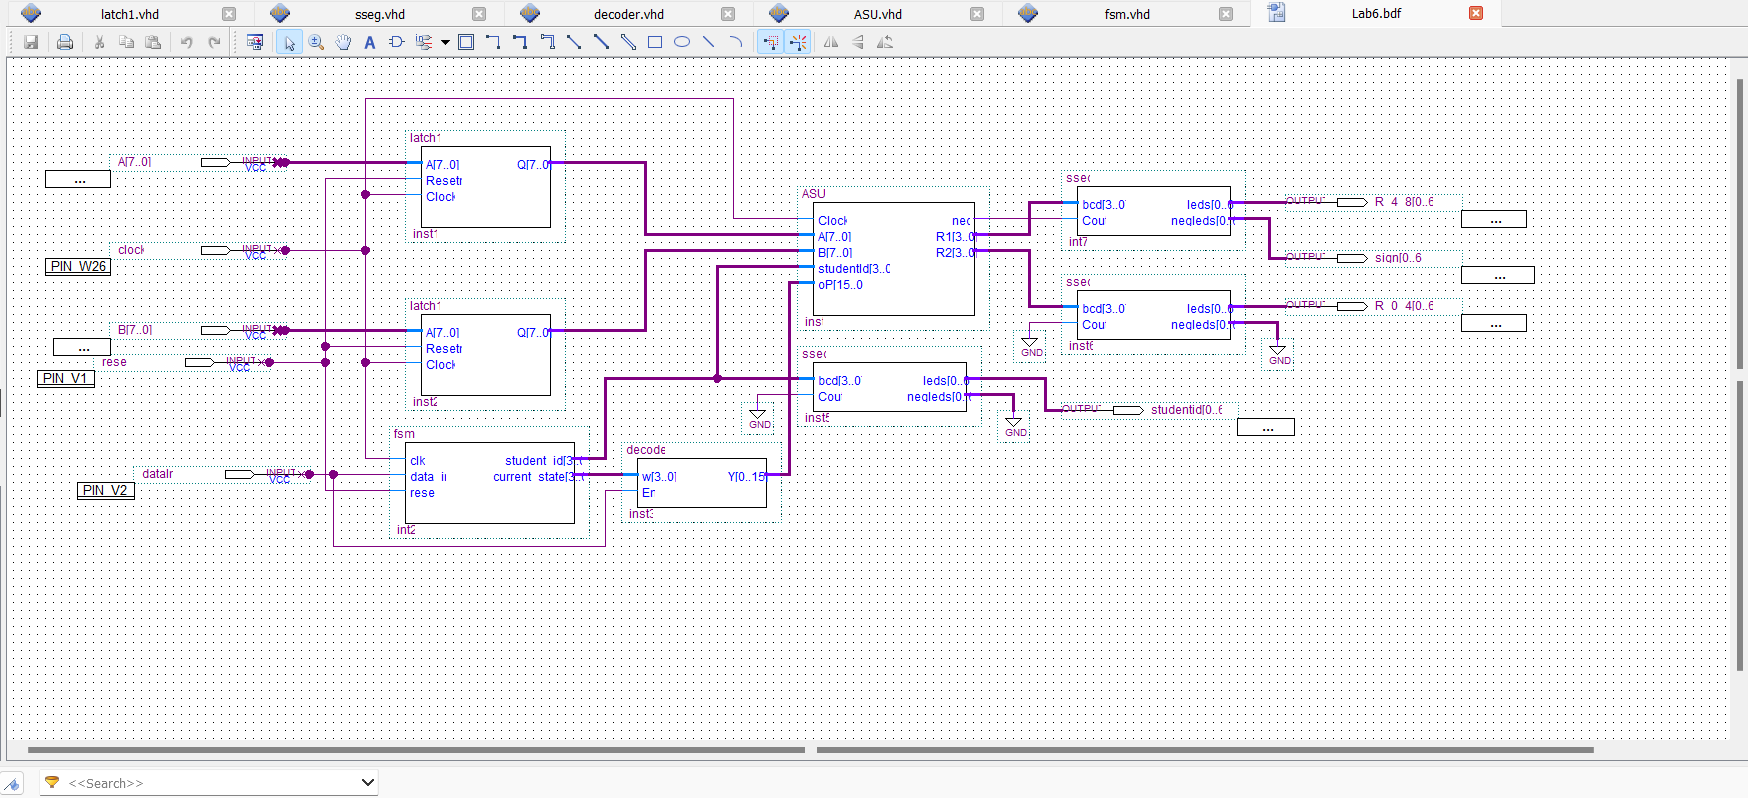
\includegraphics[width=16cm]{Pictures/BlockDiagram.png}
    \caption{{Block Diagram of the Complete Logic Circuit}}
    \label{FSM}
\end{figure}
